\documentclass[a4paper]{article}

\usepackage[T2A]{fontenc}
\usepackage[russian]{babel}
\usepackage{graphicx}
\usepackage{float}
\usepackage{hyperref}
\usepackage{amsmath, amssymb}
\usepackage{caption}
\usepackage{geometry}
\usepackage{pdfpages}
\usepackage{booktabs}
\geometry{top=2cm,bottom=2cm,left=2cm,right=2cm}

\newcommand{\minus}{\scalebox{0.75}[1.0]{$-$}}


\title{\Huge{Физика}\\ Решение Овчинкина}
\author{\huge{Евгений Турчанин}}
\date{}

\begin{document}

\begin{center}
\textsc{Санкт-Петербургский национальный исследовательский институт информационных технологий, механики и оптики\\[3mm]
Физический факультет} \\[3mm]

\end{center}
\vspace{5mm}
\line(1,0){\textwidth}
\begin{center}
\textbf{ЛАБОРАТОРНАЯ РАБОТА №1.03\\}
\textbf{"Изучение центрального соударения двух тел"}
\end{center}
\vspace{2mm}
\line(1,0){\textwidth}
\vspace{5mm}
\begin{minipage}{0.4\textwidth}
    Группа: Z3144 \\
    Студент: Евгений Турчанин\\
    \vspace{1mm}
\end{minipage}
\hfill
\vspace{1mm}
\line(1,0){\textwidth}




\section{\bf{Цели}}

\begin{enumerate}
	\item Исследование упругого и неупругого центрального соударения
тел на примере тележек, движущихся с малым трением.
	\item Исследование зависимости ускорения тележки от приложенной
силы и массы тележки.
\end{enumerate}


\section{\bf{Теоретическое введение}}
\textbf{Часть 1}\\
Рассмотрим абсолютно упругое центральное соударение двух
тел массами $m1$ и $m2$.При таком соударении в замкнутой систе
ме двух тел выполняются законы сохранения импульса и энергии.
Пусть до соударения движется только первое тело, тогда уравнения
законов имеют вид
\begin{equation}
	\begin{cases}
	m_1\vec v_{10}=m_1\vec v_1+m_2\vec v_2\\
	\dfrac{m_1 v^2_{10}}{2}=\dfrac{m_1 v^2_1+m_2 v^2_2}{2}
	\end{cases}
\end{equation}

где $\vec v_{10}$ – скорость первого тела до удара, $\vec v_1$ и $\vec v_2$ – соответственно,
скорости первого и второго тел после удара. Считая скорость $\vec v_{10}$
известной, найдем скорости обоих тел после удара. Пусть условия
соударения таковы, что после удара оба тела продолжают двигаться параллельно той прямой, по которой двигалось первое тело до удара.
\begin{figure}[H]
\begin{center}
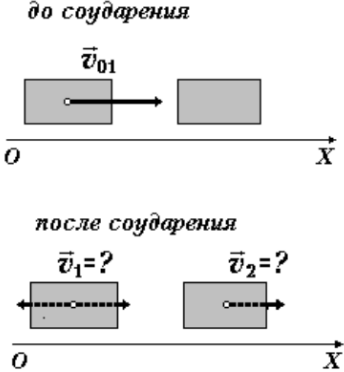
\includegraphics[scale=0.5]{pick1.png}
\caption {Тела до соударения и после}
\end{center}
\end{figure}
Введем координатную ось $OX$ , сонаправленную с вектором $v_{10}$
(см. Рис. 1). Для проекций скоростей $v_{1x}$, $v_{2x}$ из уравнений (1)
получим систему двух уравнений:

\begin{equation}
	\begin{cases}
		m_1v_{10}=m_1v_{1x}+m_2v_{2x}\\
		\dfrac{m_1v^2_{10}}{2}=\dfrac{m_1v^2_{1x}+m_2v^2_{2x}}{2}
	\end{cases}
\end{equation}
Умножим все слагаемые второго уравнения на два, и перенесем
налево в обоих уравнениях слагаемые, характеризующие импульс и
энергию первого тела:

\begin{equation}
	\begin{cases}
		m_1(v_{10}-v_{1x})=m_2v_{2x}\\
		m_1(v^2_{10}-v^2_{1x})=m_2v^2_{2x}
	\end{cases}
\end{equation}
После удара скорость первого тела должна изменится. Поэтому
содержимое скобок в левых частях уравнений (3) отлично от нуля,
и для упрощения системы можно поделить левые и правые части
нижнего уравнения на соответствующие части верхнего уравнения.
Результат деления сделаем вторым уравнением системы:
\begin{equation}
	\begin{cases}
		m_1(v_{10}-v_{1x})=m_2v_{2x}\\
		v_{10}+v_{1x}=v_{2x}
	\end{cases}
\end{equation}
Отсюда нетрудно найти окончательные выражения для скоростей
\begin{equation}
	\begin{cases}
		v_{1x}=\dfrac{(m_1-m_2)v_{10}}{m_1+m_2}\\
		v_{2x}=\dfrac{2m_1v^2_{10}}{m_1+m_2}
	\end{cases}
\end{equation}
Из первого уравнения (5) следует, что в зависимости от соотно
шения масс первое тело после соударения может:\\
а) продолжить движение вперед ($m1$ > $m2$, $v_{1x}$ > 0);\\
б) остановится ($m1$ = $m2$, $v_{1x}$ = 0);\\
в) поменять направление движение на противоположное ($m_1$ <
$m_2$, $v_{1x}$< 0).\\
При абсолютно неупругом соударении рассмотренных выше тел,
оба тела после удара двигаются как одно целое с суммарной массой.
В этом случае законы сохранения импульса и энергии принимают
вид:
\begin{equation}
	\begin{cases}
		m_1\vec v_{10}=(m_1+m_2)\vec v\\
		\dfrac{m_1 v^2_{10}}{2}=\dfrac{(m_1+m_2) v^2}{2}+W_{\text{пот}}
	\end{cases}
\end{equation}

Здесь $\vec v$ – скорость тел после соударения , $W_{\text{пот}}$ – потери механической энергии при соударении.\\
В первом уравнении (6) равенство векторов означает равенство
их модулей, и для модуля скорости тел после соударения из этого
уравнения находим:
\begin{equation}
	v=\dfrac{m_1v_{10}}{m_1+m_2}
\end{equation}

Подставив во второе уравнение системы (6) вместо скорости $v$
правую часть уравнения (7), получим следующее выражение для
потерь механической энергии при соударении:
\begin{equation}
	W_{\text{пот}}=\dfrac{m_1m_2v^2_{10}}{2(m_1+m_2)}
\end{equation}
Относительные потери механической энергии при неупругом соударении вычисляются по формуле:
\begin{equation}
	\dfrac{W_{\text{пот}}}{\dfrac{m_1v^2_{10}}{2}}=
	\dfrac{m_2}{m_1+m_2}
\end{equation}

В качестве соударяющихся тел в лабораторной работе выступают две тележки, скользящие с малым трением по горизонтальному
рельсу.\\
\textbf{Часть 2}\\
\begin{figure}[H]
\begin{center}
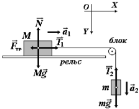
\includegraphics[scale=0.5]{pick2.png}
\caption {Система из тележки и гирьки, соедененных нитью}
\end{center}
\end{figure}
Рассмотрим систему, состоящую из тележки M и гирьки m, соединенных невесомой нерастяжимой нитью (см. Рис. 2). Тележка с небольшим трением скользит по горизонтальному рельсу. Масса
блока, через который перекинута нить,пренебрежимо мала.\\
Уравнения второго закона Ньютона для тележки и гирьки, соответственно, имеют вид:
\begin{equation}
	M\vec a_1=M\vec g + \vec N + \vec T_1 + \vec F_{\text{тр}}\\
	m\vec a_2=m\vec g + \vec T_2
\end{equation}
Здесь $\vec a_1$, $\vec a_2$ – ускорения тележки и гирьки;
$\vec N$ – сила реакции опоры,
$\vec T_1$,$\vec T_2$ – силы натяжения нити, $\vec F_{\text{тр}}$ – сила трения. Из-за
нерастяжимости нити модули обоих ускорений равны друг другу,
обозначим их одной буквой: $a_1=a_2=a$. Из-за невесомости нити и
блока можно также принять, что силы натяжения с обеих сторон
блока равны друг другу: $T_1=T_2=T$.
Для проекций векторов на координатные оси из уравнения (10)
получаем:

\begin{equation}
	\begin{cases}
		OY: N=Mg\\
		OX: Ma=T-F_{\text{тр}}
	\end{cases}
\end{equation}
из уравнения (11):
\begin{equation}
	OY: ma=mg-T
\end{equation}
Из второго уравнения системы (12) следует, что сила натяжения
нити и ускорение тележки связаны соотношением:
\begin{equation}
T=Ma+F_{\text{тр}}
\end{equation}
Если сила трения не изменяется во время эксперимента, то из соотношения (14) зависимость $T(a)$ является линейной. Угловой коэффициент этой зависимости равен массе $M$ тележки, а значение
силы натяжения при нулевом ускорении равно силе трения $F_{\text{тр}}$.\\
Формулы для вычисления различных величин:
\begin{equation}
p_{10x} = m_1 \cdot v_{10x},\quad p_{1x} = m_1 \cdot v_{1x}, \quad p_{2x} = m_2 \cdot v_{2x}
\end{equation}\\
\begin{equation}
	\delta_p=\Delta p_x/p_{10x}=\dfrac{(p_{1x}+p_{2x})}{p_{10x}}-1
\end{equation}
\begin{equation}
	\delta_W=\Delta W_k/W_{k0}=\dfrac{m_1v^2_{1x}+m_2v^2_{2x}}{m_1v^2_{10x}}-1
\end{equation}
Где $\delta_p$ - относительное изменение импульса, $\Delta_W$ - относительное изменение энергии.\\
\begin{equation}
\delta p_{\text{ср}} = \frac{1}{N} \sum_{i=1}^{N} \delta p_i
\end{equation}
\begin{equation}
\delta W_{\text{ср}} = \frac{1}{N} \sum_{i=1}^{N} \delta W_i
\end{equation}
\begin{equation}
\Delta \overline{\delta p} = t_{\alpha \text{дов},N} \sqrt{\frac{ \sum_{i=1}^{N} (\delta p_i - \delta p_{\text{ср}})^2 }{N(N - 1)}},
\end{equation}
\begin{equation}
\Delta \overline{\delta W} = t_{\alpha \text{дов},N} \sqrt{\frac{ \sum_{i=1}^{N} (\delta W_i - \delta W_{\text{ср}})^2 }{N(N - 1)}}.
\end{equation}
\begin{equation}
	\delta_W^{(T)}=-\dfrac{W_{\text{пот}}}{\dfrac{m_1v^2_{10}}{2}}=-\dfrac{m_2}{m_1+m_2}
\end{equation}
\begin{equation}
a=\dfrac{(v_2^2-v_1^2)}{2(x_2-x_1)}, T=m(g-a)
\end{equation}


\section{\bf{Схема работы}}
\begin{figure}[H]
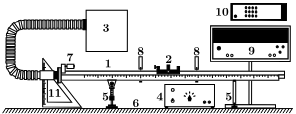
\includegraphics[width=\textwidth]{pick3.png}
\caption{Общий вид экспериментальной установки}
\end{figure}
Общий вид экспериментальной установки для первой части ра-
боты изображен на Рис. 3. В состав установки входят:
1. Рельс с сантиметровой шкалой на лицевой стороне\\
2. Сталкивающиеся тележки\\
3. Воздушный насос\\
4. Источник питания насоса ВС 4-12\\
5. Опоры рельса\\
6. Опорная плоскость (поверхность стола)\\
7. Фиксирующий электромагнит\\
8. Оптические ворота\\
9. Цифровой измерительный прибор ПКЦ-3\\
10. Пульт дистанционного управления прибором ПКЦ-3\\

\section{\bf{Данные}}
\begin{figure}[H]
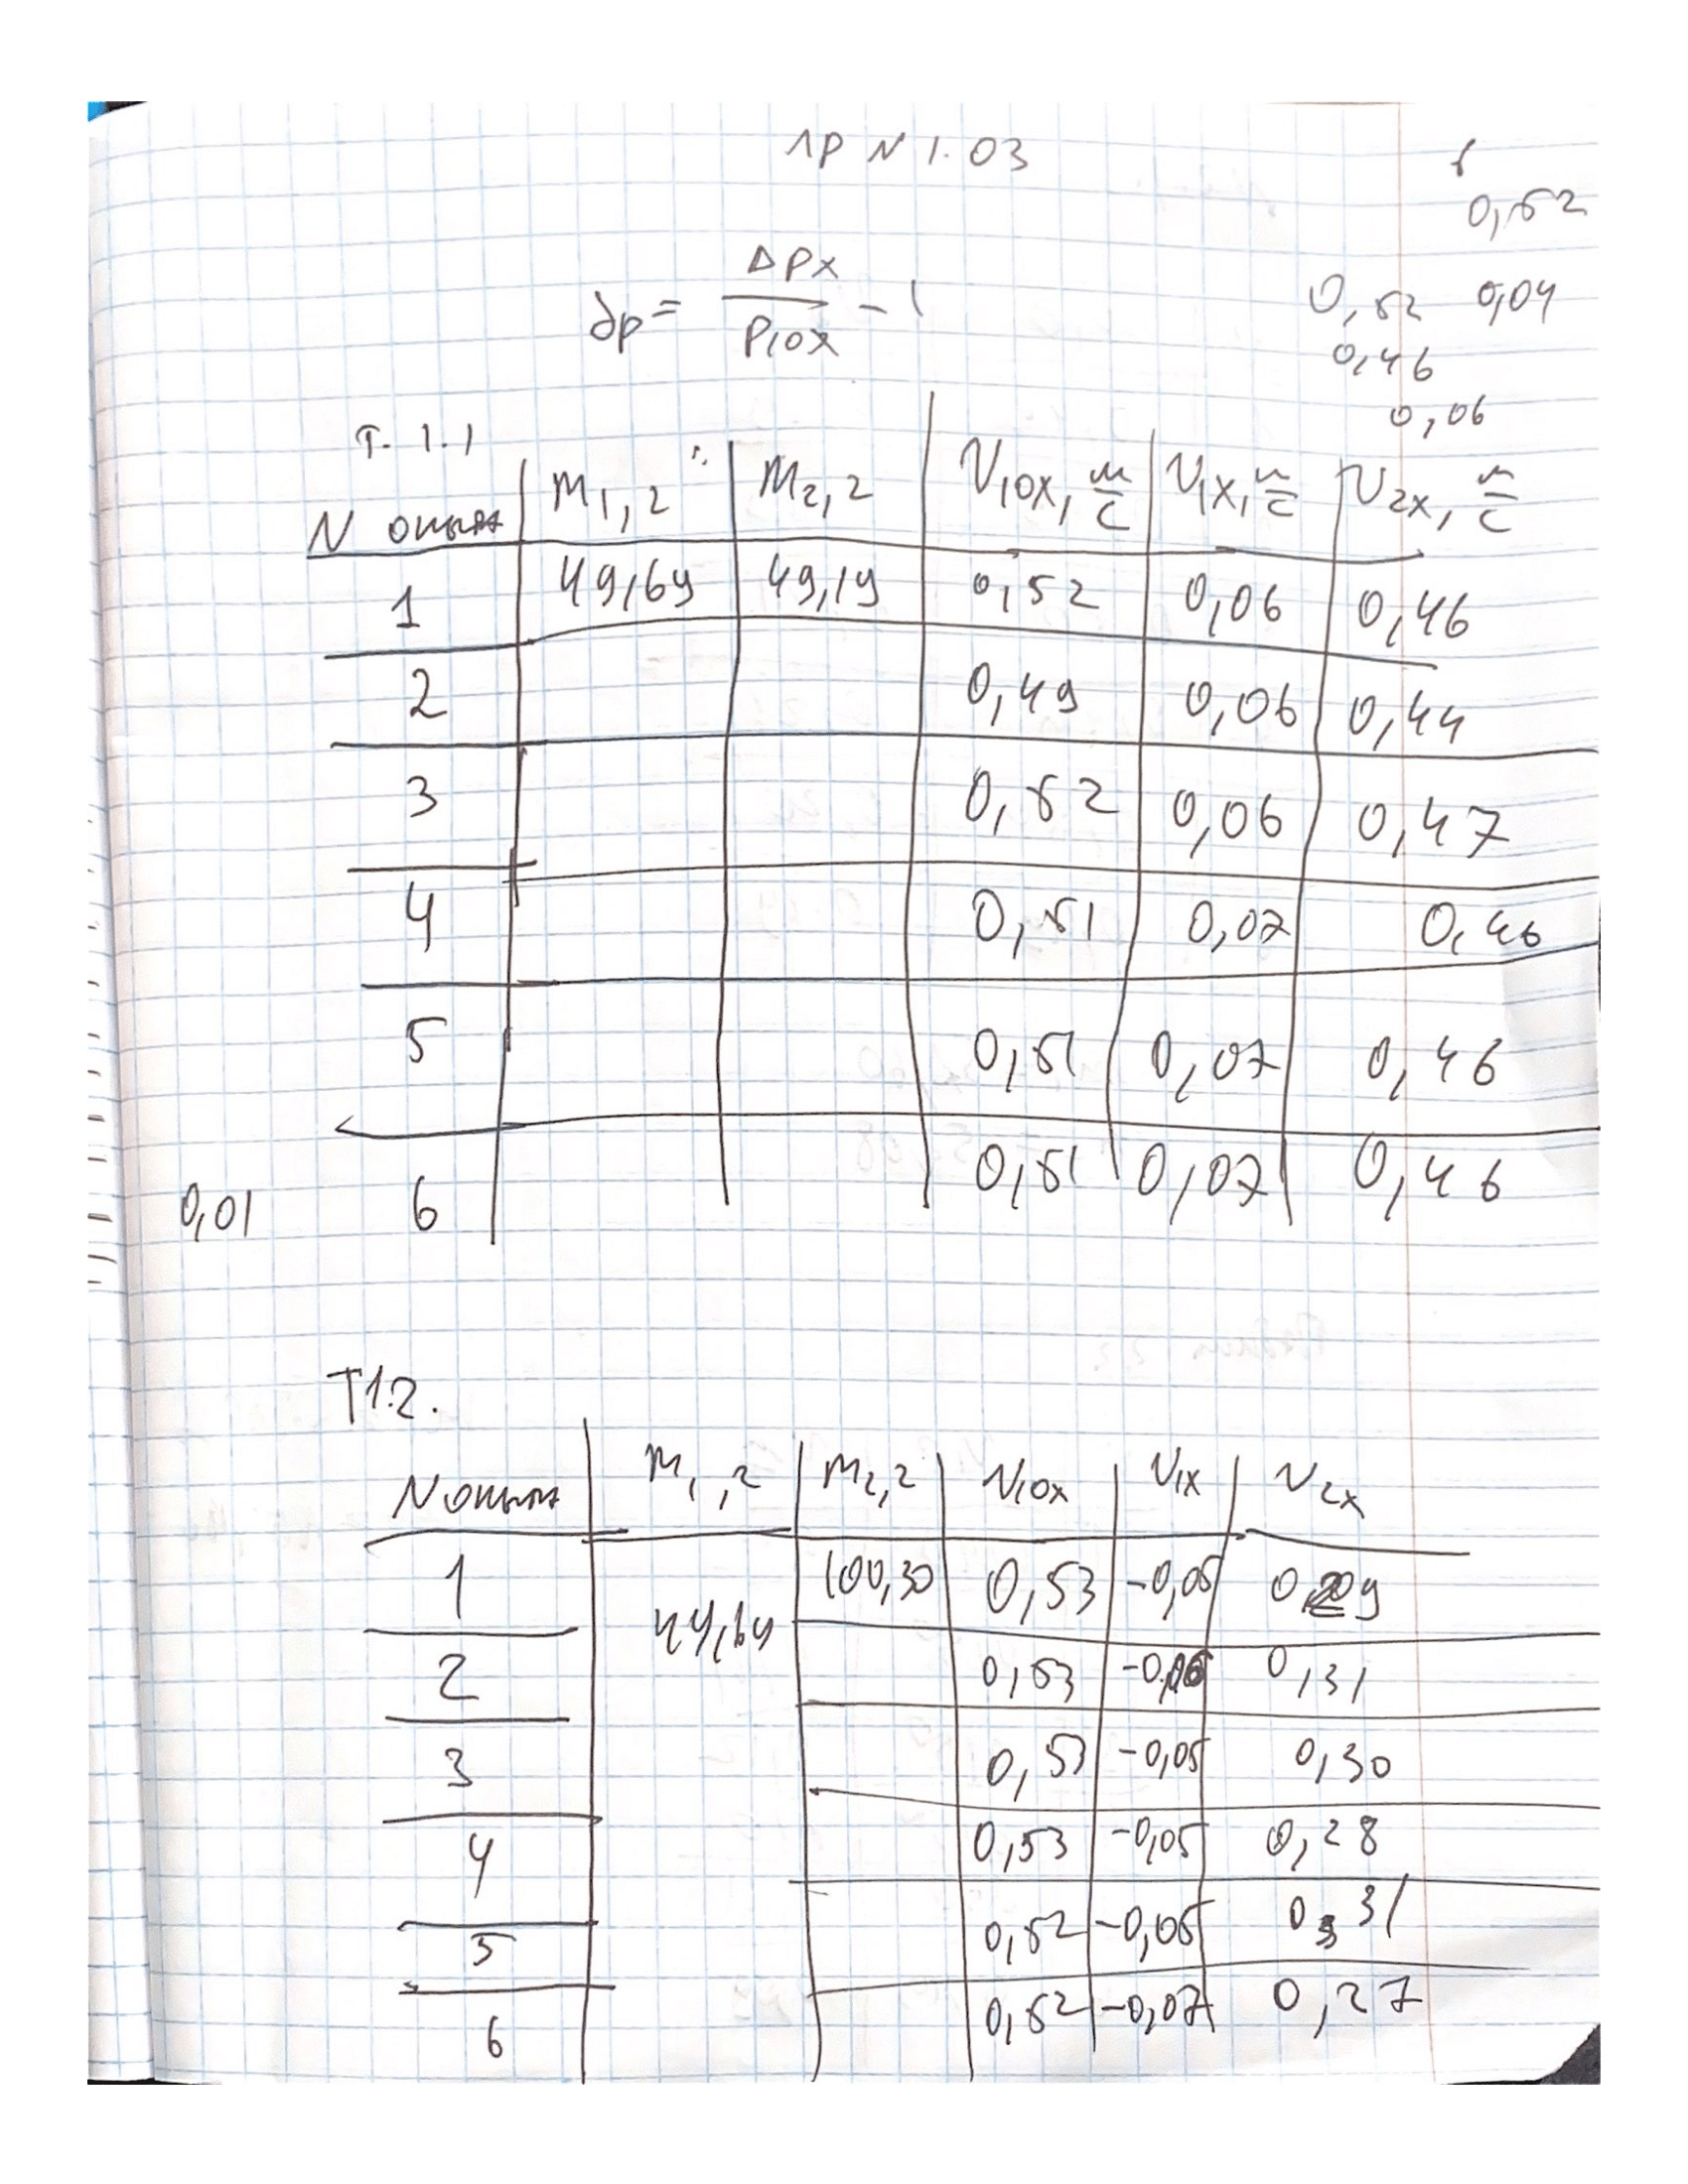
\includegraphics[width=\textwidth, scale=0.5]{1-1.png}
\caption{Данные}
\end{figure}
\begin{figure}[H]
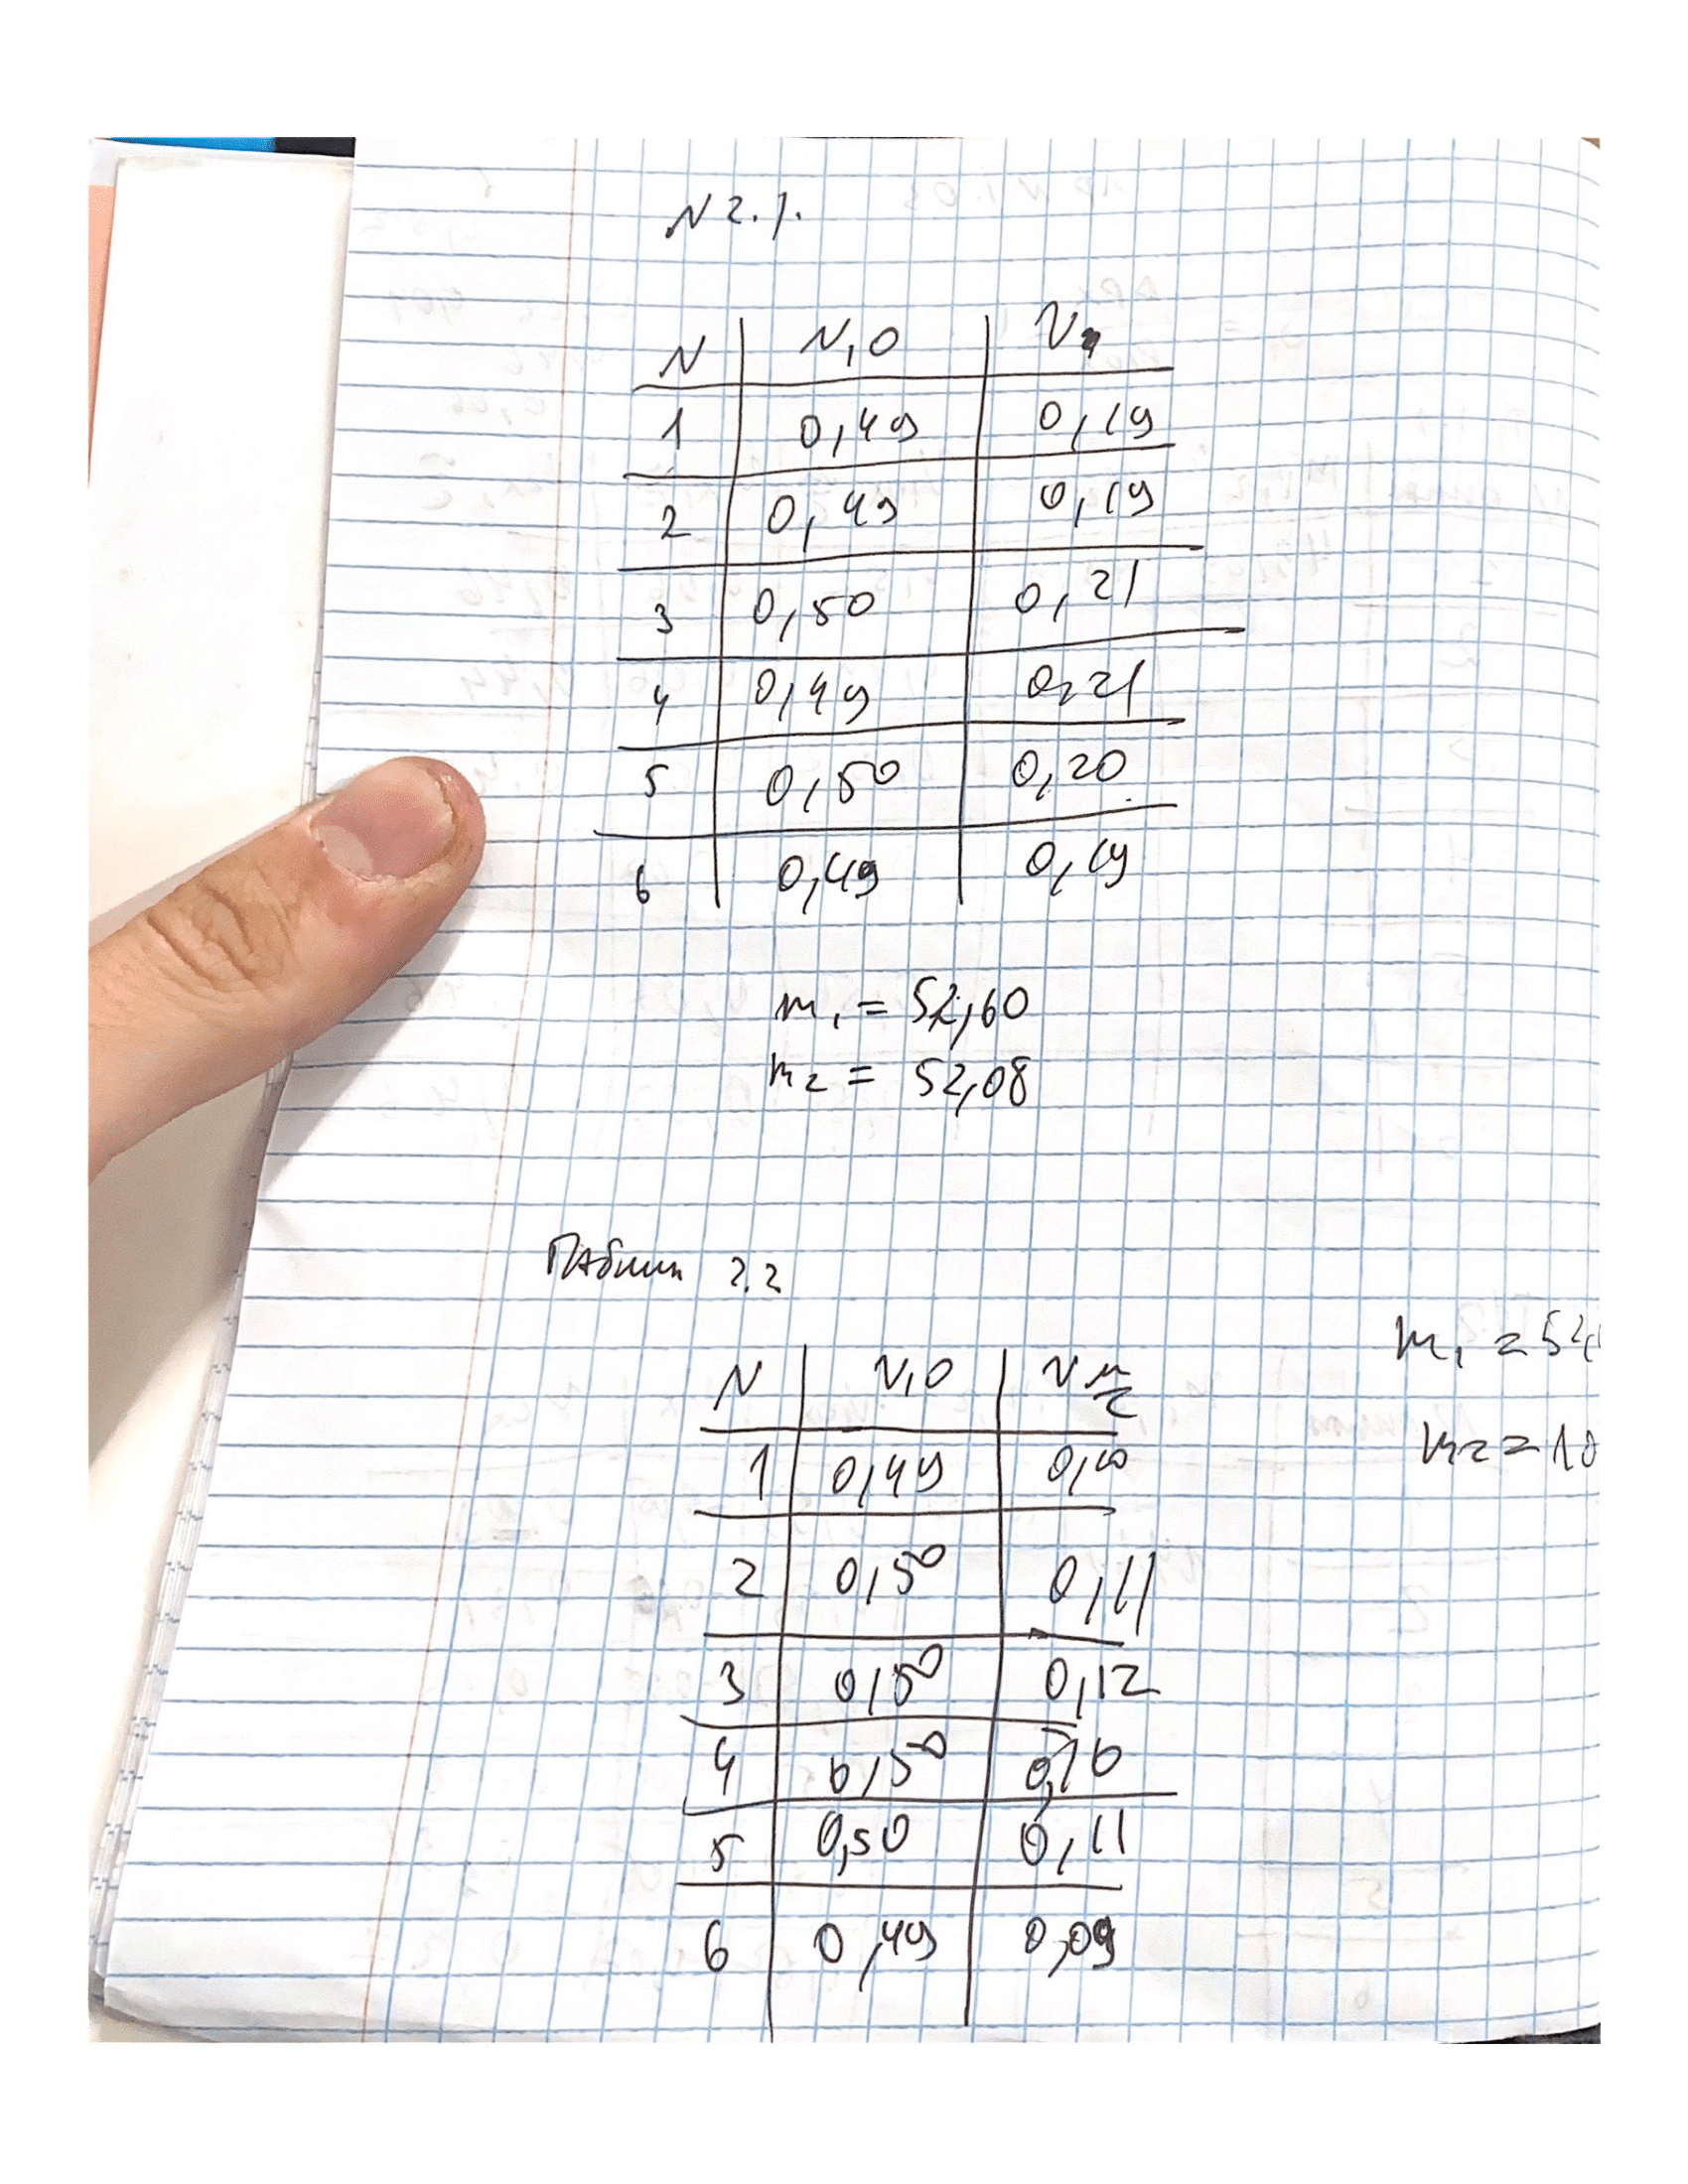
\includegraphics[width=\textwidth, scale=0.5]{1-2.png}
\caption{Данные}
\end{figure}
\begin{figure}[H]
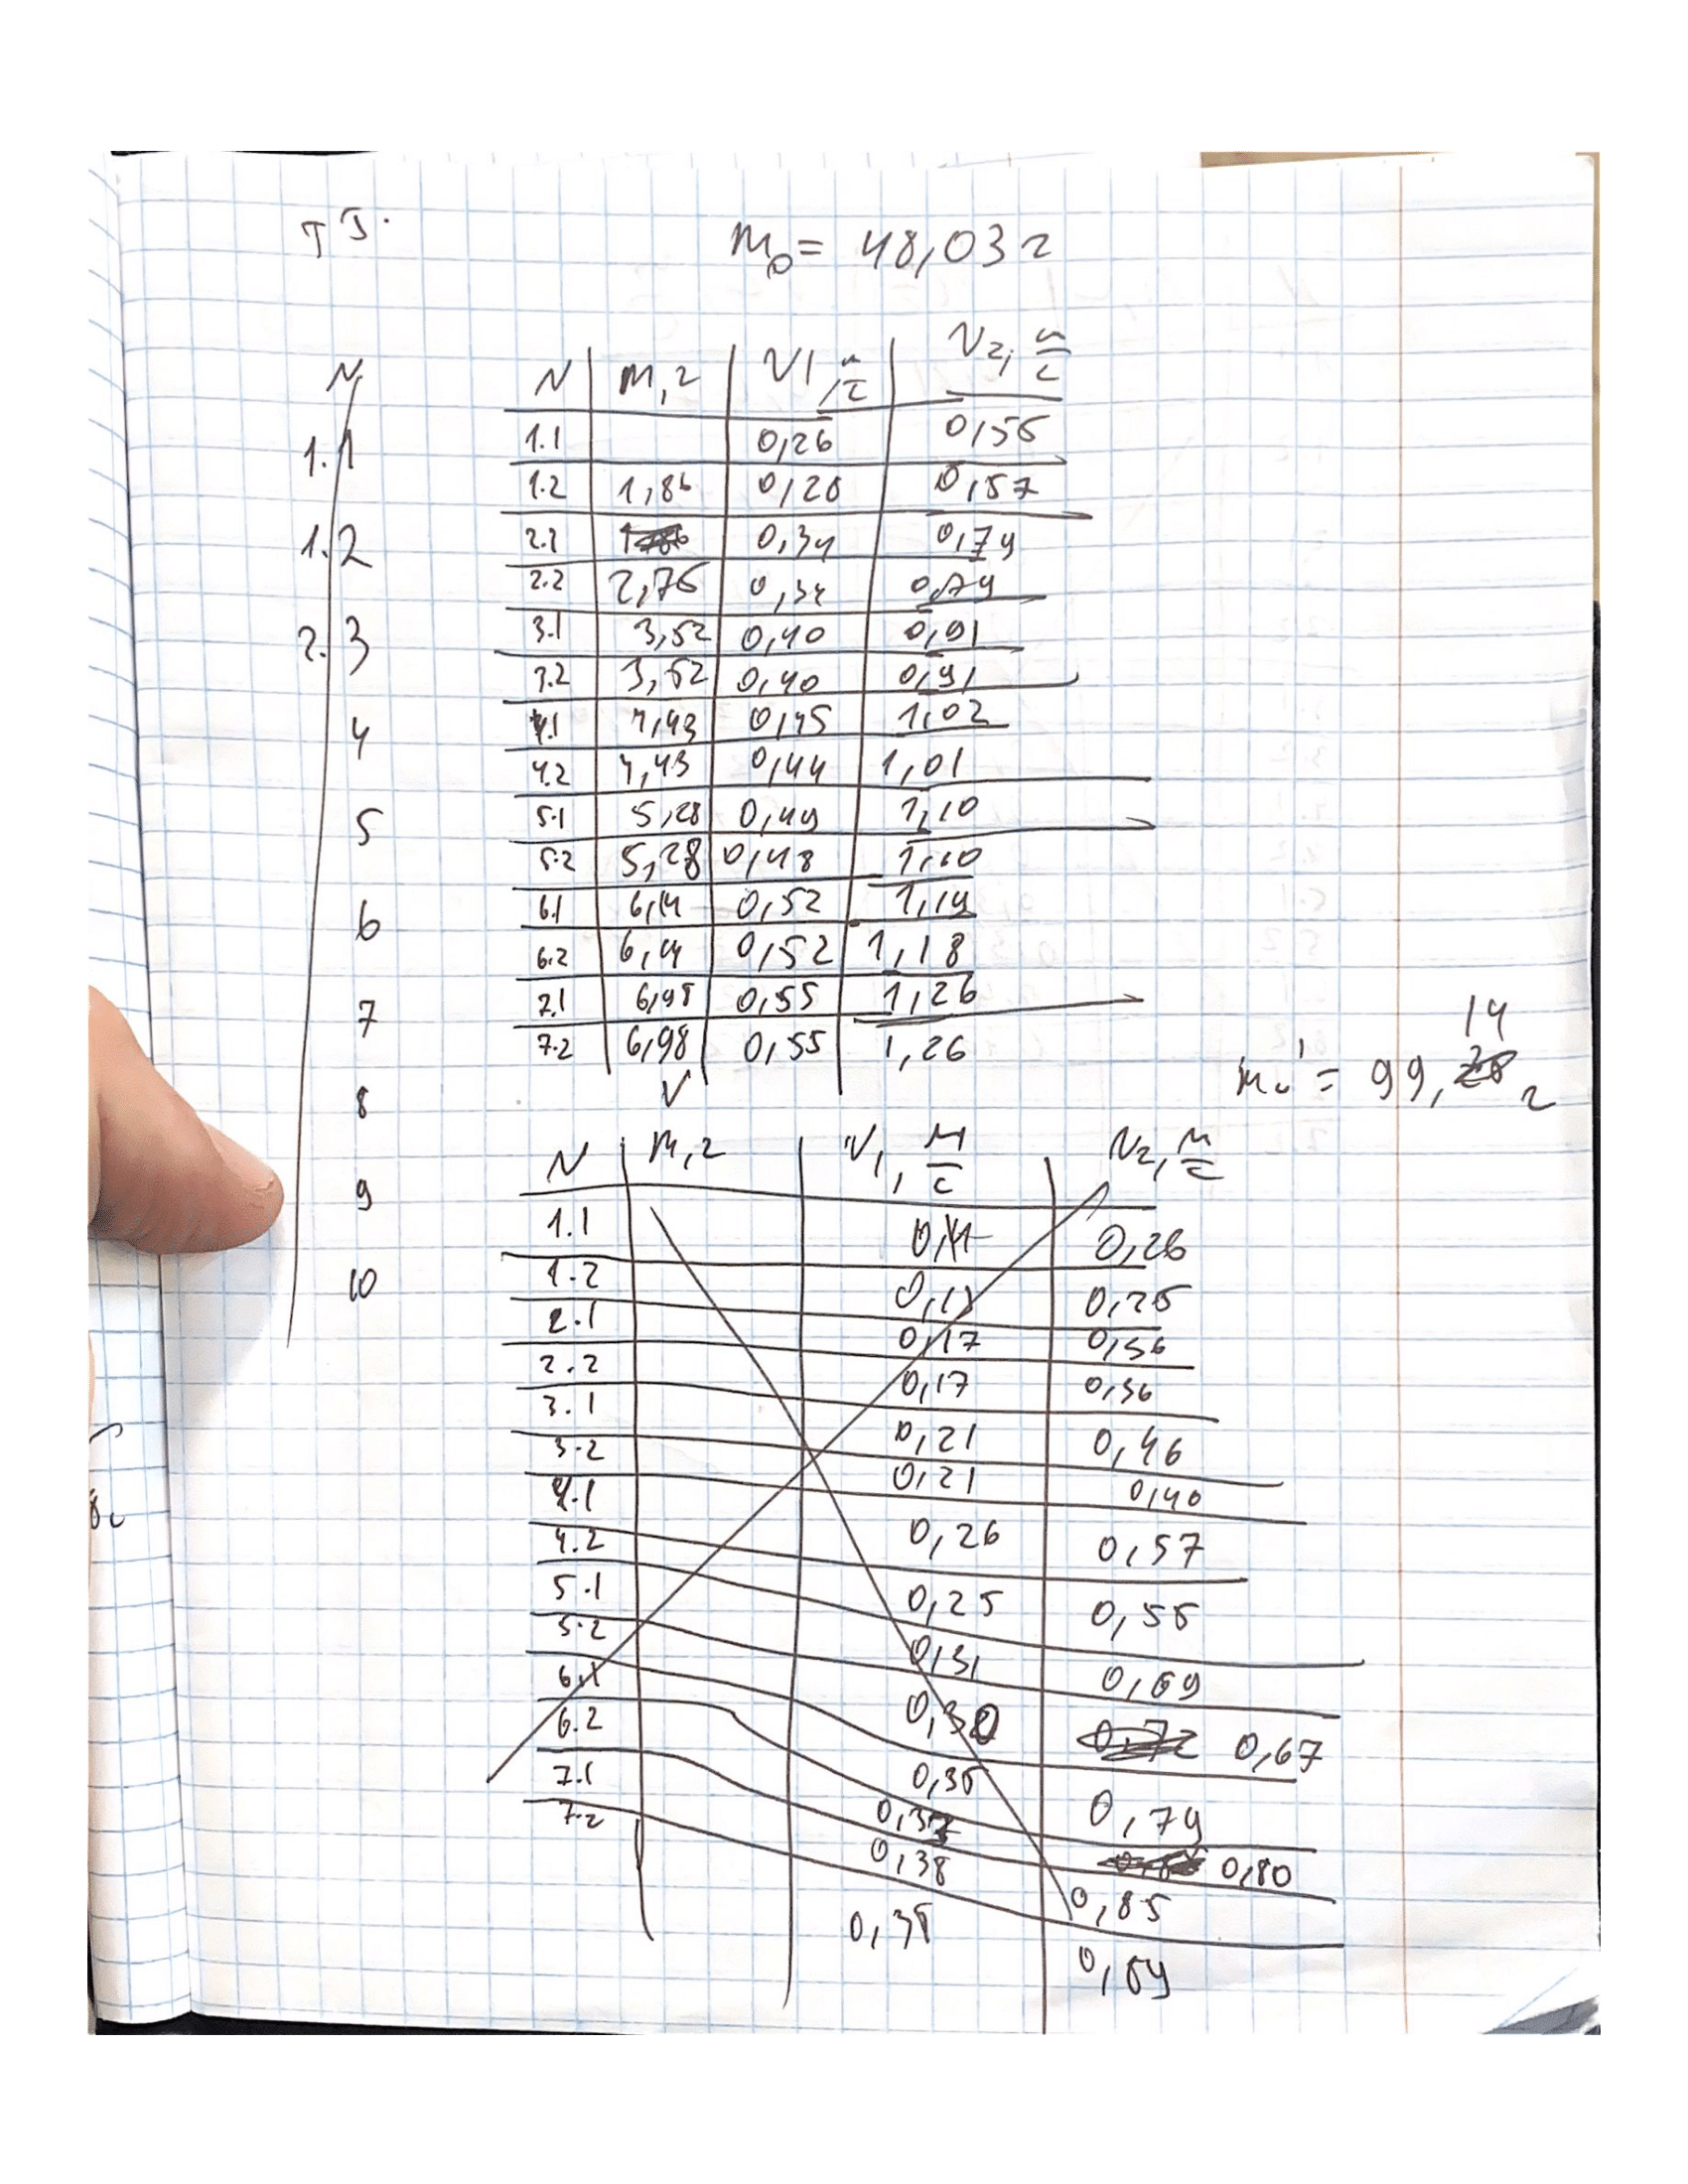
\includegraphics[width=\textwidth, scale=0.5]{1-3.png}
\caption{Данные}
\end{figure}
\begin{figure}[H]
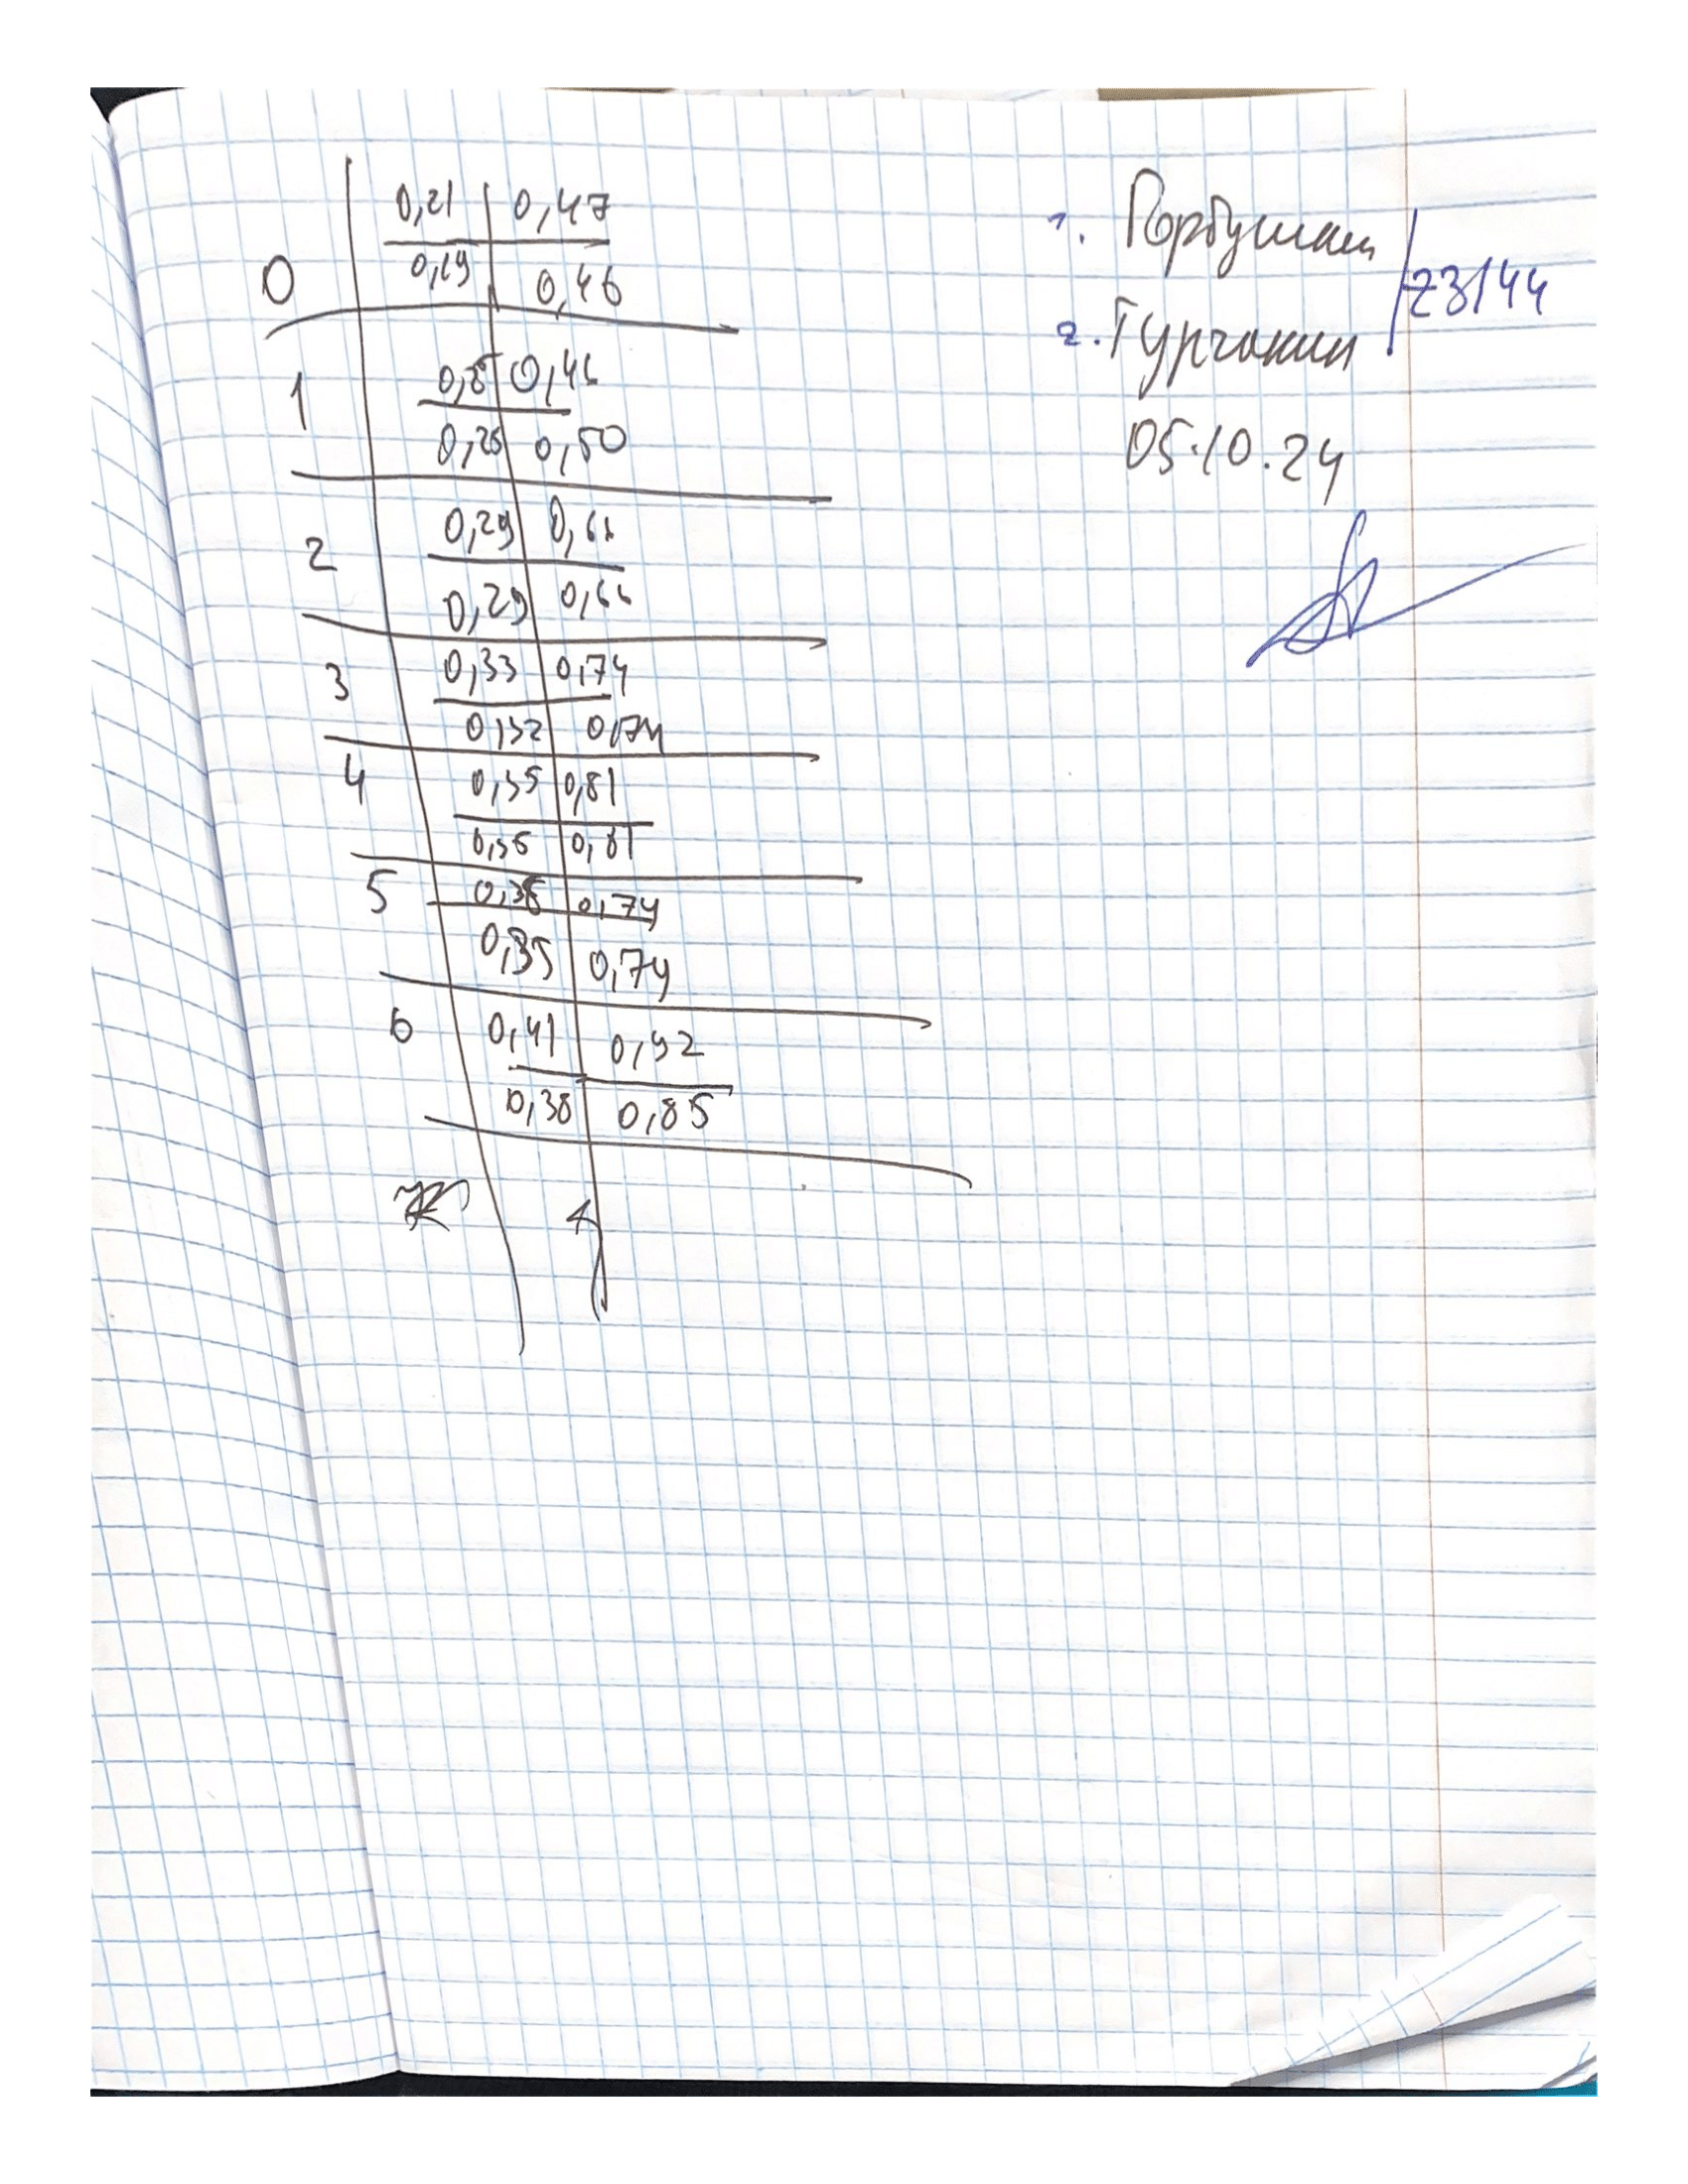
\includegraphics[width=\textwidth, scale=0.5]{1-4.png}
\caption{Данные}
\end{figure}


\section{\bf{Результаты прямых измерений и их обратоки}}


\begin{center}
\textbf{При упругом соударении:}
\begin{align*}
\text{Доверительный интервал для } \delta_p &: -0.038 \pm 0.013 \\
\text{Доверительный интервал для } \delta_W &: -0.164 \pm 0.006 \\
\text{Доверительный интервал для } \delta_p &: -0.826 \pm 0.0389\\
\text{Доверительный интервал для } \delta_W &: -0.814 \pm 0.0205\\
\text{Теоретическое отклоление энергии } \delta_W^{(T)} &: -0.549\\
\end{align*}

\textbf{При неупругом соударении:}
\begin{align*}
\text{Доверительный интервал для } \delta_p &: -0.190 \pm 0.046 \\
\text{Доверительный интервал для } \delta_W &: -0.673 \pm 0.037 \\
\text{Доверительный интервал для } \delta_p &: -0.383 \pm 0.077 \\
\text{Доверительный интервал для } \delta_W &: -0.86 \pm 0.033 \\
\text{Теоретическое отклоление энергии } \delta_W^{(T)} &: -0.655\\
\end{align*}
\end{center}
График зависимости силы натяжения от ускорения для легкой и утяжеленной тележки:
\begin{figure}[H]
\begin{center}
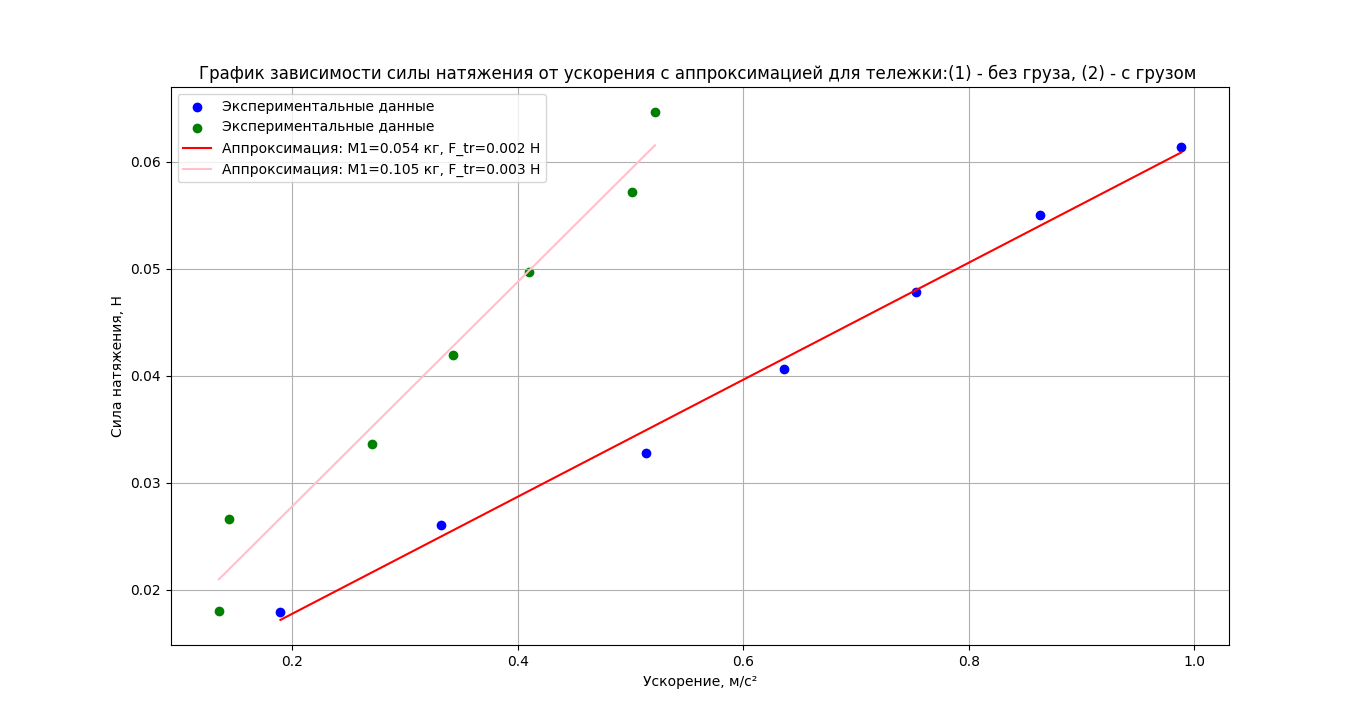
\includegraphics[width=\textwidth, scale=0.5]{Figure_1.png}
\end{center}
\end{figure}
\textbf{Теоретические значение масс тележки и тележки с грузом:}
\begin{center}
\begin{align*}
\text{Доверительный интервал для } M1 &: 0.055 \pm 0.003 \\
\text{Доверительный интервал для } M2 &: 0.105 \pm 0.008 \\
\end{align*}
\end{center}
Массы измеренные на весах:
\begin{center}
\begin{align*}
\text{Доверительный интервал для } M1 &: 0.052\\
\text{Доверительный интервал для } M2 &: 0.104
\end{align*}
\end{center}


\section{Выводы}

\begin{itemize}
	\item Из выше приведенных данных можно сделать выводы, что эксперимент не расходится с теорией
	\item Погрешность вожет быть вызванна несколькими факторами:
	\begin{enumerate}
		\item Плохой работой насоса, из-за перегрева источника питания мог работать не на полную, вследствии чего сила трения была большей чем это требует эксперимент
		\item Изугнутость рельсы, из-за чего тележка могла терять часть скорости
		\item Из-за достаточно малого трения/изогнутости рельсы, тележку нельзя поставить без начальной скорости
	\end{enumerate}
\end{itemize}
\end{document}


